 %美赛模板:正文部分

\documentclass[12pt]{article}  % 官方要求字号不小于 12 号,此处选择 12 号字体
% \linespread{1.1}
% \bibliographystyle{plain}
% 本模板不需要填写年份,以当前电脑时间自动生成
% 请在以下的方括号中填写队伍控制号

\usepackage[2412704]{easymcm}  % 载入 EasyMCM 模板文件

\problem{C}  % 请在此处填写题号

\usepackage[english]{babel}

% \usepackage{mathptmx}  % 这是 Times 字体,中规中矩 
\usepackage{palatino}  % mathpazo 这palatino是 COMAP 官方杂志采用的更好看的 Palatino 字体,可替代以上的 mathptmx 宏包
\usepackage{pdfpages}
\usepackage{longtable}
\usepackage{graphicx}
\usepackage{caption}
\usepackage{fancyhdr}
\usepackage{booktabs}
\usepackage{hyperref}
\usepackage{tabu}
\usepackage{algorithm}
\usepackage{pdfpages}
\usepackage{lastpage}  % To reference the last page before the PDF is included
\usepackage{algorithmic}
\usepackage{threeparttable}
\usepackage{listings}
\usepackage{multicol}
\usepackage{paralist}

\graphicspath{{img/}}          % 此处{img/}为相对路径,注意加上“/”
 \let\itemize\compactitem
 \let\enditemize\endcompactitem

\newcommand{\upcite}[1]{\textsuperscript{\textsuperscript{\cite{#1}}}}
\title{Build an Army of Drones to Fight Wildfires}  % 标题

% 如需要修改题头(默认为 MCM/ICM),请使用以下命令(此处修改为 MCM)
%\renewcommand{\contest}{MCM}

 %文档开始
\begin{document}

% 此处填写摘要内容
\begin{abstract}
    
Global warming, El Niño...... With the emergence of various extreme climates,\textbf{Austral-ia's wildfires} occur more frequently. The greenhouse gases emitted after combustion have exacerbated global warming, which seems to have entered an endless loop. At the same time, hundreds of millions of lives have been killed in the fire, which makes us sad. In order to better control wildfires, we modeled the \textbf{distribution of drones} assisting in the observation to achieve the best balance between economy and efficiency.

Several models are established: Model I: Rasterized Multi-Objective Optimization Model; Model II: Model Verification Simulated by Poisson Process; Model III: Hovering Model Based on Tabu Search, etc.

For Model I: According to the \textbf{heat map} about distribution of fires in Victoria in recent years, we found that the main fire areas are the plains along the eastern coast. Inspired by weights and \textbf{Multi-Objective Optimization} algorithms, we built a brand-new model to find the best location for EOCs and draw up a suitable hover position and reconnaissance route for the drone. Based on the different positions of the fire site, calculate the maximum num-ber of two types of drones and their ratio. The results are shown in Figure 9.

For Model II: This model is actually a supplement to Model I. In the Model I, the fire only appeared in a small area, and there was a possibility of extreme fire events in the study area. Combining the data about nearly half a century and using the \textbf{Poisson Distribution }to obtain the probability and mathematical expectation, it can be concluded that 2.99431 ex-treme fire events may occur in the next ten years, which is approximately considered to be 3 times. After that, use the mobile EOC to deal with extreme fire events, and utilize the method of Model I to rebuild the drone network to find out what equipment costs need to be increased. Due to the diversity of the results, it will be shown in section 6.2.

For Model III: To tackle the problem of how to optimize the hover position of drones in different terrains, the \textbf{Tabu Search }algorithm (TS) is a good choice. Using the Tabu Search algorithm can make the hover position of the drones achieve the global optimal ef-fect under different terrain conditions. Since drone signals are severely interfered in urban areas, the reasonable distribution of EOCs enables it to quickly network to respond to sud-den urban fires. The obstruction of mountainous terrain restricts the drone's flying range. Therefore, dividing the area into blocks and managing them separately can effectively im-prove efficiency. $\frac{{(x \cdot \gamma) \cdot \theta + 8}}{{6 \cdot \theta}}$

Finally, sensitivity analysis of the mathematical expectation of extreme fire events $\xi$ shows that our model is not sensitive to changes in $\xi$ , that is, it can be applied to areas with different extreme fire invents. Meanwhile, robustness of our model has also been tested. While adding 5\% random disturbance to $d_{k i}^{\alpha}$  and $d_{k i}^{\beta}$ , the maximum time error is 3.2657\%. 

% 美赛论文中无需注明关键字。若您一定要使用,
% 请将以下两行的注释号 '%' 去除,以使其生效
\vspace{5pt}  %mm	毫米	1 mm = 2.845 pt   pt 点	1 pt = 0.351 mm;此处为Keywords与Abstract正文额外相隔的距离(1.5cm)
\textbf{Keywords}: Fighting Wildfires; Multi-Objective Optimization; Poisson Distribution; Tabu Search Algorithm; Sensitivity Analysis

\end{abstract}

\maketitle  % 生成 Summary Sheet


% 生成目录

\tableofcontents  



% Chapter 1: Introduction

\section{Introduction}

\subsection{Background}
If you are a fan in competitive sports games like tennis, you might have heard a lot of the word “Momentum”. When a player has momentum, they seem to control the dominance of the match, wielding the match's rhythm and flow. Novak Djokovic, a record-breaking tennis player, described this in his saying: “… if you have the mental ability to stay strong, stay patient and \textbf{confident} and just have \textbf{belief} in the right moments, then you get a win, you know.”

However, momentum is not stationary; you probably have witnessed momentum being lost or stolen from a player during a match, entirely changing the outcome. Momentum can switch to the other player within the blink of an eye and stun unsuspecting players and spectators. This is especially spectacular during the 2023 Wimbledon Gentlemen’s final between Carlos Alcaraz and Novak Djokovic (Figure 1). In this match, Djokovic completely dominated the first set with a score of 6 – 1, displaying enormous momentum. However, this quickly shifted to Alcaraz in the third set, where he won 6 - 1, before Djokovic regained control in the fourth set with a 6 - 3 win. Finally, in the late stages of the fifth set, the momentum swung once again, and Alcaraz secured victory with a score of 6 - 4.

But where \textbf{exactly} did that momentum come from? Despite its recognized impact, momentum has remained largely a qualitative factor and rooted in the subjective experience of spectators and self-perception of athletes. The question, then, is whether this intangible force can be analyzed and systematically understood through mathematical methods. If this proves feasible, it has the potential to greatly enhance the strategies used by competitive tennis players and coaches and, by extension, athletes and coaches in various sports.

\begin{figure}[htbp]
	\centering
	\begin{minipage}{0.5\textwidth}
	\centering  %图表居中

\includegraphics[width=.95\textwidth]{carlos-alcaraz.jpg} %图片的名称或者路径之中有空格会出问题 
\caption{Carlos Alcaraz (Left) and Novak Djokovic (Right) at Wimbledon \cite{1}} % 图片标题 
\label{fig:Fire Situation} % 图片标签,可以不写
	\end{minipage}\hfill
	\begin{minipage}{0.45\textwidth}
	\centering  %图表居中
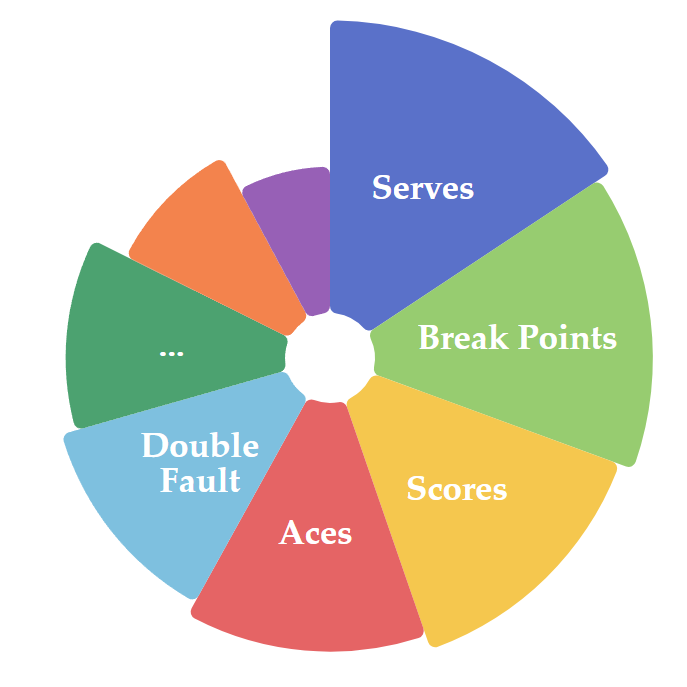
\includegraphics[width=.6\textwidth]{data-given.png} %图片的名称或者路径之中有空格会出问题 
\caption{Data Aspects Provided by Wimbledon\_featured\_matches.csv} % 图片标题 
\label{fig:Fire Situation} % 图片标签,可以不写
	\end{minipage}
\end{figure}

\subsection{Problem Analysis}

Momentum is a \textit{phenomenon}, which means it is an outcome of a wide range of factors, including psychological states, like confidence and mental toughness, to external conditions like the current state of the match. To analyze and build a robust model that measures the momentum of players in competitive tennis, it is crucial to cover these factors extensively. Specifically, our model should be capable of completing the following tasks:

\begin{enumerate}[\bfseries (1)]
\setlength{\parsep}{0ex} %段落间距
\setlength{\topsep}{2ex} %列表到上下文的垂直距离
\setlength{\itemsep}{1ex} %条目间距
\item Evaluate the quatitive degree how one player is performing better than the other player at any given point in the match, and illustrate the changes of such degree visually.
\item Based on extensive factors, including the flow of match, the model should quantify the concept of "momentum" in tennis matches, and identify potential indicators that could predict shifts in momentum. To address the coach’s skeptism, the model needs to be compared to a null model that assumes outcomes are random (e.g., based on point-by-point win probabilities without momentum).
\item Finally, the developed "momentum" model should be tested on other matches from the different matches, including women's matches, to exhibit its predictive accuracy and generalizability, and identify any limitations or additional factors that may need to be incorporated. 
\end{enumerate}

\subsubsection{Capturing the Match's Flow}
To compare the performance ratings between the two players, we can use the data provided in Wimbledon\_featured\_matches.csv that describe the explicit match information, such as whether a player was serving or at a break point, etc. (shown in Figure 2); but we also need to consider other implicit information that has significant impact on the state of the match, for example, whether a player has a high scoring streak. Other unimportant information, potentially the speed of the serve, needs to be neglected to ensure model's simplicity and robustness. This inherently requires \textbf{feature engineering}: to extract and construct feature variables that capture both explicit and implicit aspects that control the flow of the match.

Since our model aims to dynamically assess the match's state as it unfolds, it requires a granular focus on the ebb and flow of the game, taking into account both minor and major developments at any given moment. For example, the player may have an advantage in games won, but when the other player just scored a break point, that player could be performing much better at that specific time. Therefore, to scope the data to recently played points, the \textbf{sliding window} technique can be employed; to handle older scores and progressively update the model as the match goes on, introduction of a \textbf{forgetting factor} would be applicable, as illustrated in Figure 3. The remaining work would be finding an appropriate model to map these parameters to the performance or the win rate of a player. 

\begin{figure}[htbp]  %h此处,t页顶,b页底,p独立一页,浮动体出现的位置
	\centering  %图表居中
	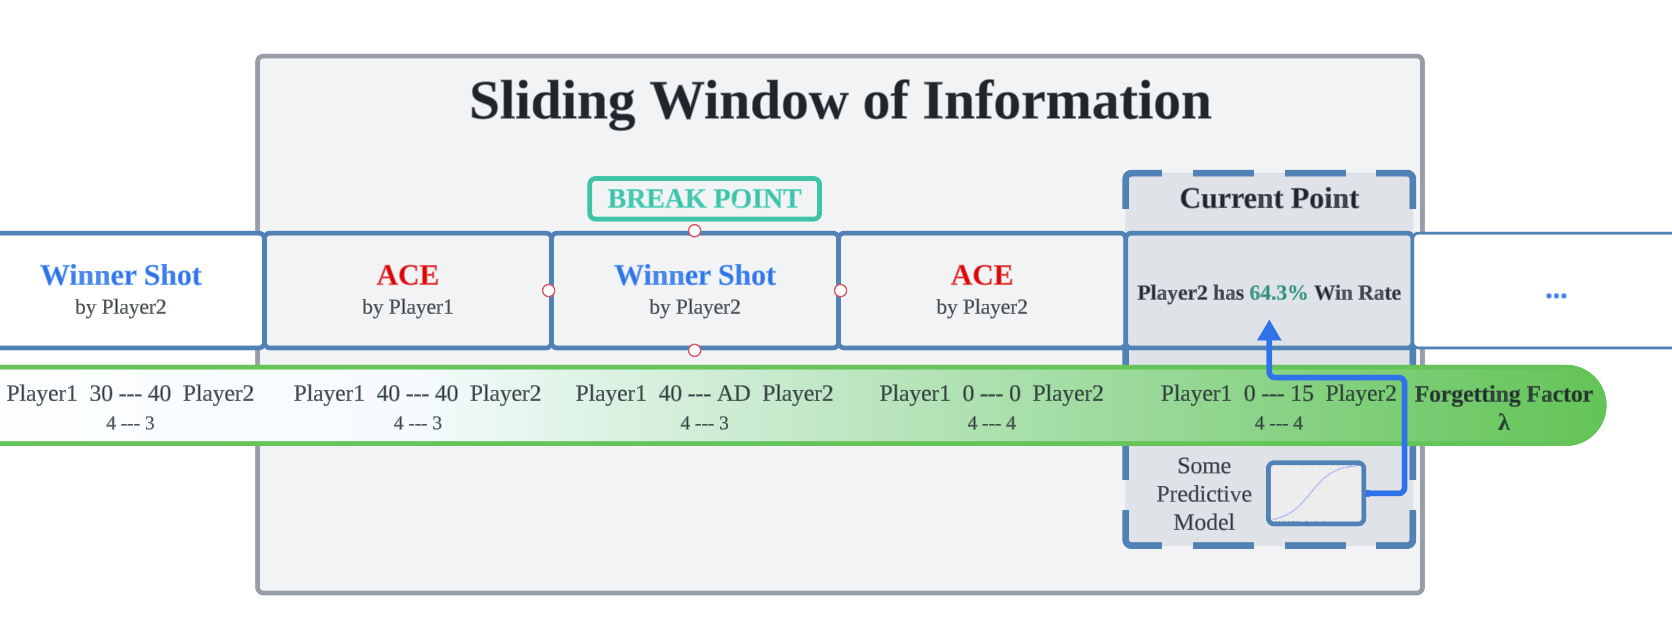
\includegraphics[width=.85\textwidth]{sliding-window.png} %图片的名称或者路径之中有空格会出问题 
	\caption{\centering Information Is Constrained by Sliding Window and Forgetting Factor. (Note that the data in this graph is for display purposes only.)} % 图片标题 
\end{figure}


\subsection{Literature Review}
This question is mainly about mobilizing cluster drones to extinguish wildfires. In re-cent years, research on optimization algorithms for UAV(drone) cluster path planning is very hot, Generally, it can be divided into two parts, the \textbf{Swarms of UAVs' Path Planning Model} and the \textbf{Swarms of UAVs' Path Planning Optimization Algorithm}, this section mainly discusses the models that have been proposed.

\begin{itemize}
\setlength{\parsep}{0ex} %段落间距
\setlength{\topsep}{2ex} %列表到上下文的垂直距离
\setlength{\itemsep}{1ex} %条目间距  这三句如果删除就是各条贴在一起
\item First of all, in terms of the dimensionality of the space: In\cite{2} HU et al. sets the plan-ning space to three dimensions. However, in order to simplify the model, more authors tend to consider the space as two dimensions\cite{3}.
\item Secondly, in terms of the method of planning space: the commonly used methods in-clude Grid Method\cite{4}, Road Sign Method, and Artificial Potential Fields Method.
\item Finally, the objective function of the UAV Cluster Path Planning Model generally uses flight distance, threat cost, etc. For example, Xu et al.\cite{5} takes the weighted sum of threat cost and time cost as the optimization target. What's more, Constraints often in-clude self-constraints and environmental constraints, such as flight speed and geo-graphic altitude.
\item The strengths and weaknesses of the planning space can be visually presented and is shown below:
\end{itemize}

\begin{figure}[htbp]  %h此处,t页顶,b页底,p独立一页,浮动体出现的位置
\centering  %图表居中
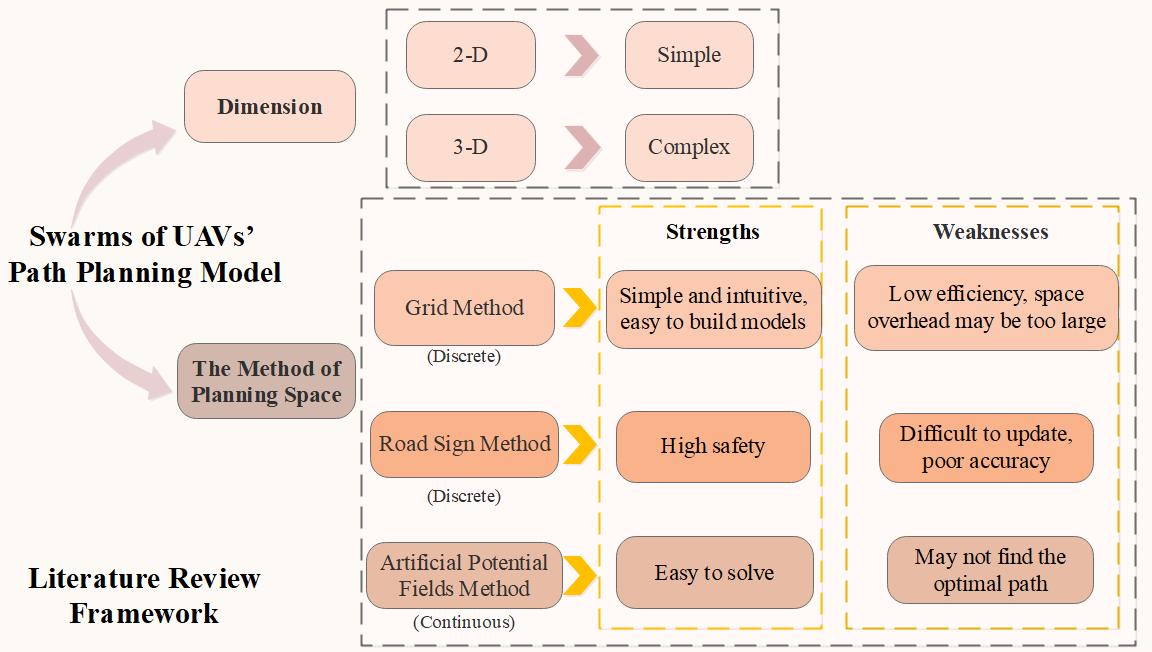
\includegraphics[width=.85\textwidth]{Literature_Review.png} %图片的名称或者路径之中有空格会出问题 
\caption{Literature Review Framework} % 图片标题 
\end{figure}

\subsection{Our Work}
In this paper, we seek to mathematically model the flow of momentum across a tennis match, and use it to provide insights to benefit tennis coaches and atheletes across the world. It is our belief that a practical and inclusive mathematical framework would greatly help the tennis community in understanding the concept of momentum to improve performance, strategy, and training methodologies. Through extensive investigation and research in the field of tennis, our main model, the \textbf{Dynamic Tennis Momentum Analyzer (DTMA)}, integrates a comprehensive set of features and use a variety of statistical methods to achieve this goal. The building of this model can be overall described as follows:
\begin{enumerate}[\bfseries (1)]
    \setlength{\parsep}{0ex} %段落间距
    \setlength{\topsep}{2ex} %列表到上下文的垂直距离
    \setlength{\itemsep}{1ex} %条目间距
    \item To capture the flow of match in real-time, we constructed the CourtSense model as a sub-model of DTMA. The model starts by applying a Sliding Window machanism to a set of extracted features; these features are passed into the core Progressive Logisic Model that use the set of principal factors to predict the winning chance of the point; due to the real-time progression of the competition, a Forgetting Factor is added to dynamically update this model to reflect the most recent match status. 
    \item The mixture of the two drones is given and the extreme fire events is considered;
    \item Based on the verification model simulated by Poisson process and the hovering model based on Tabu Search, this article effectively demonstrates the validity and applicability.
\end{enumerate}
In order to avoid complicated description, intuitively reflect our work process, the flow chart is shown in Figure 3:

\begin{figure}[htbp]  %h此处,t页顶,b页底,p独立一页,浮动体出现的位置
\centering  %图表居中
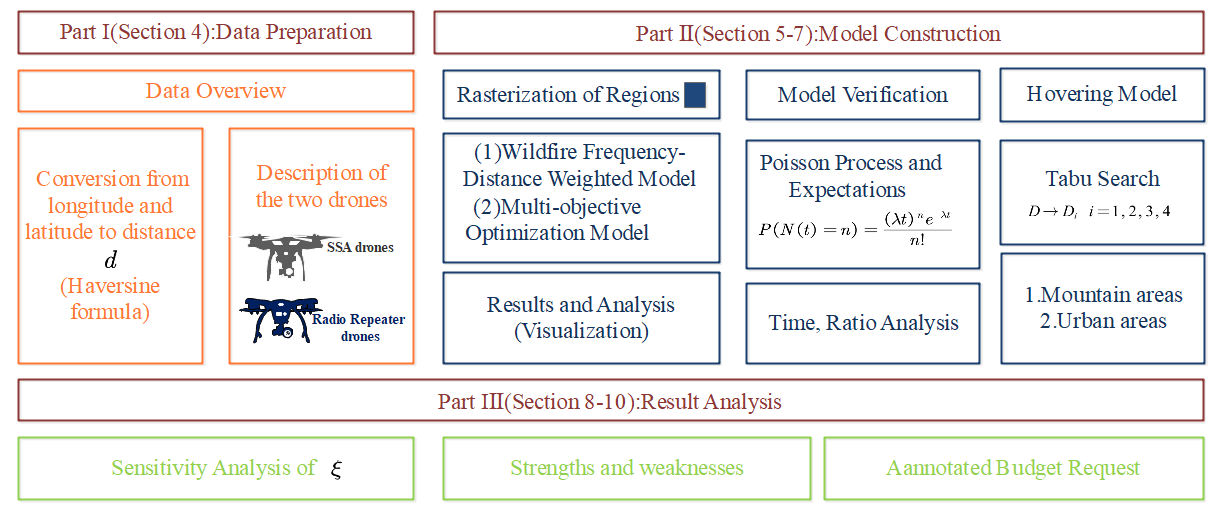
\includegraphics[width=.9\textwidth]{Flow_Chart.png} %图片的名称或者路径之中有空格会出问题 
\caption{Flow Chart of Our Work} % 图片标题 
\end{figure}
\vspace{-0.8cm}



% 2. Assumptions 

\section{Assumptions and Explanations}
Considering that practical problems always contain many complex factors, first of all, we need to make reasonable assumptions to simplify the model, and each hypothesis is closely followed by its corresponding explanation:

\begin{enumerate}[\bfseries \textit{Assumption} 1:]
	\item \textbf{Only the influence of terrain on the drone is considered, and other factors such as temperature, humidity, and atmosphere are ignored.}\\
	\textbf{\textit{Explanation: }}The UAV's radiation communication range is only affected by terrain factors, and other factors are minimal. In fact, these factors affect each other, but in order to simplify the model ,we ignore the interactions between these factors.
	\item \textbf{The location of the EOC can be deployed around the fire due to an emergency.}\\
	\textbf{\textit{Explanation: }}The position of the EOC is not clearly given in the question. So, we assume that EOC can be set in a fire-free area around the wildfire site, since the glossary of the problem said that mobile EOC can be deployed near the site of an emergency.
	\item \textbf{The "boots-on-the-ground" forward teams can be approximated as near the fire site.}\\
	\textbf{\textit{Explanation: }}The actual movement of the team is very complicated, and it is difficult to accurately calculate its position. Therefore, it is assumed that the squad is near the fire field and the drone arrives at the fire field to establish a connection with the squad.
	\item \textbf{The collected data can be considered reliable and can reflect the changing laws of the Victorian wildfire.}\\
	\textbf{\textit{Explanation: }}The historical Victorian wildfire data, latitude, longitude and other data come from authoritative websites, such as the official website of FEC in Australia and NASA, with high accuracy.
\end{enumerate}
Additional assumptions are made to simplify analysis for individual sections. These assumptions will be discussed at the appropriate locations.




% 3. Notation

\section{Notations}
Some important mathematical notations used in this paper are listed in Table 1. 
\begin{table}[htbp]
\begin{center}
\caption{Notations used in this paper}
\begin{tabular}{c l}
\toprule[2pt]
\multicolumn{1}{m{3cm}}{\centering Symbol} & \multicolumn{1}{m{8cm}}{\centering Description }\\
\midrule
$x_i$ & Longitude within the i-th Wildfire Grid \\
$y_i$ & Latitude within the i-th Wildfire Grid \\
$\varOmega _i$ & The area of the i-th grid\\
$d_{ki}$ & the distance $d_{ki}$ between the k-th roaming grid and the i-th grid \\
$SC_k$ & Score for evaluating the k-th wildfire grid \\
\vspace{5pt}%公式间有点挤,空一些
$x^{( \alpha )}_{ki}$ & the $SSA_\alpha$ drone sent by the k-th EOC to the i-th wild-fire grid\\
\vspace{3pt}
$x^{( \beta )}_{ki}$ & the $RR_\beta$ drone sent by the k-th EOC to the i-th wildfire grid\\
$t_{fly}^{\delta}$ & The flight time of drones\\
\bottomrule[2pt]
\end{tabular}\label{tb:notation}
 \begin{tablenotes}
        \footnotesize
        \item[*] *There are some variables that are not listed here and will be discussed in detail in each section. %此处加入注释*信息
      \end{tablenotes}
\end{center}
\end{table}
\vspace{-1cm}%在\end{table}下加一行\vspace{-1cm} 其中-1的作用是缩短与下方文字距离的 切记!必须是负数





% 4. Model

\section{CourtSense Model: Judging the State of the Match}
The CourtSense model aims to capture the current state of the match by predicting the outcome of the next unplayed point, using available match information. First, we need to apply feature engineering to the given data to extract useful features.

\subsection{Feature Engineering}

\subsubsection{Data Processing}
The data provided by the problem (Wimbledon\_featured\_matches.csv) is a comprehensive dataset that contains the complete match information, including scores, serve details, point details which are all applicable to analyze the state of the match. After a thorough inspection of the data, we find that the data is clean and usable. However, these are all explicit match information and is limited to a specific point, for example, whether this player is serving, what is the ratio of scores, etc. We think that more temporal features like whether this player is leading in score are more direct in describing the match’s status; hence we added them to the feature set. These additional features are included in Table 2.


\begin{table}[htbp]
	\centering  % Use \centering instead of the center environment to avoid extra vertical space
	\caption{Added Match Information}
	\resizebox{\textwidth}{!}{% Adjusted the resizebox command
		\begin{tabular}{ccc}  % Simplified column specification since you're centering all cells
			\toprule[2pt]
			\multicolumn{1}{m{4cm}}{\centering \textbf{Column Name}} &
			\multicolumn{1}{m{8cm}}{\centering \textbf{Description}} & 
		\multicolumn{1}{m{5cm}}{\centering \textbf{Example Value}} \\ 
	\midrule
	p1\_streak & The winning losing streak of player 1 up until that point & 5, 0, -3 \\
	p2\_streak & The winning losing streak of player 2 up until that point & 3, 0, -5 \\ 
	p1\_leading & Whether p1 is leading in score & 1 (leading), 0, -1 \\
	p2\_leading & Whether p1 is leading in score & -1 (losing), 0, 1 \\
	p1\_leading\_game & Whether p1 is leading in game & 1, 0, -1 \\
	p2\_leading\_game & Whether p1 is leading in game & -1, 0, 1 \\
	p1\_leading\_set & Whether p1 is leading in set & 1, 0, -1 \\
	p2\_leading\_set & Whether p1 is leading in set & -1, 0, 1 \\
	\bottomrule[2pt]
\end{tabular}
}
\end{table}

These features, representing nuanced indicators of the current state of the match, are better to feed into the model than raw scores for simplicity and accuracy. For example, the winning streak is a direct reflection of the player's current performance and momentum.

Moreover, for the data columns like '\textit{game\_victor}' that represent the winner of the game (or set), we split them into 2 columns to be player-specific. For each point \( i \) in the match, we transform, for example, the \textit{game\_victor} column into two player-specific columns, \( V_{p1}^{(i)} \) and \( V_{p2}^{(i)} \), defined as:
\[
V_{p1}^{(i)} = 
\begin{cases} 
	1 & \text{if \textit{game\_victor} = 1 at point } i  \\
	-1 & \text{if \textit{game\_victor} = 2 at point } i \\
	0 & \text{if if \textit{game\_victor} = 0 at point } i
\end{cases}
\]

\[
V_{p2}^{(i)} = 
\begin{cases} 
	1 & \text{if \textit{game\_victor} = 2 at point } i \\
	-1 & \text{if \textit{game\_victor} = 1 at point } i \\
	0 & \text{if if \textit{game\_victor} = 0 at point } i
\end{cases}
\]
This procedure ensures these data can be modeled as their respective performance.  

Finally, we discarded other rather unimportant or redundant information for the match, such as the raw score information, the speed of the serve (which cannot be used for points already in play when predicting point outcomes), unforced errors (not an indicator of player's performance), and information about net points. These choices are made after conducting a thorough research on related Sports Analytics in the field of tennis \cite{2}\cite{3}\cite{4}. The remaining features alongside the constructed features can be used as raw input data for our model.

\subsubsection{Sliding Window Mechanism}
We recognize that the current state of the match is heavily influenced by the temporal features of, not only for the current point, but also the last few points. For example, if the player ran a long distance in the past few point rounds, they will carry more amount of fatigue, influencing the player's performance of the current point. Or if the player has just won a break point, they will gain much more confidence in their coming plays. Therefore, by employing a sliding window mechanism, the model can utilize the temporal features on the most recent and relevant data points, ensuring that the analysis remains sensitive to the current state of play and the immediate history before it. This is described in the formula below:

Let \( F_{t} \) and \( F_{nt} \) represent the sets of temporal and non-temporal features, respectively. For a given point in time \( t \), the combined feature set \( F^{(t)} \) is given by:

\[
F^{(t)} = S_{t}^{(t-1)} \cup F_{nt}^{(t)}
\]
where

\[
S_{t}^{(t-1)} = \sum_{i=t-3}^{t-1} F_{t}^{(i)}
\]
represents the sum of temporal features of last 3 points played, and \( F_{nt} \) represents the non-temporal features at the current point \( t \). So far, we have acquired a granular and exhaustive features that completely describe the match's status at a specific point and is ready to be fed into our Progressive Logistic Model - the core of the CourtSense model.

\subsection{Progressive Logistic Model}
To effectively capture the dynamic flow of a tennis match, we introduce the Progressive Logistic Model. This model is designed to predict the outcome probability of the current point, providing a real-time assessment of the match's status and the relative performances of the players. The Progressive Logistic Model utilizes a multivariate logistic regression framework, due to its suitability for binary outcome prediction (e.g., point won or lost) and its ability to output probabilities based on multiple features; furthermore, combined with the Forgetting Factor, the model is capable of progressively updating the model according to the latest match information as the match unfolds. The general process of this model is depicted in Figure 3. 

\begin{figure}[htbp]  %h此处,t页顶,b页底,p独立一页,浮动体出现的位置
	\centering  %图表居中
	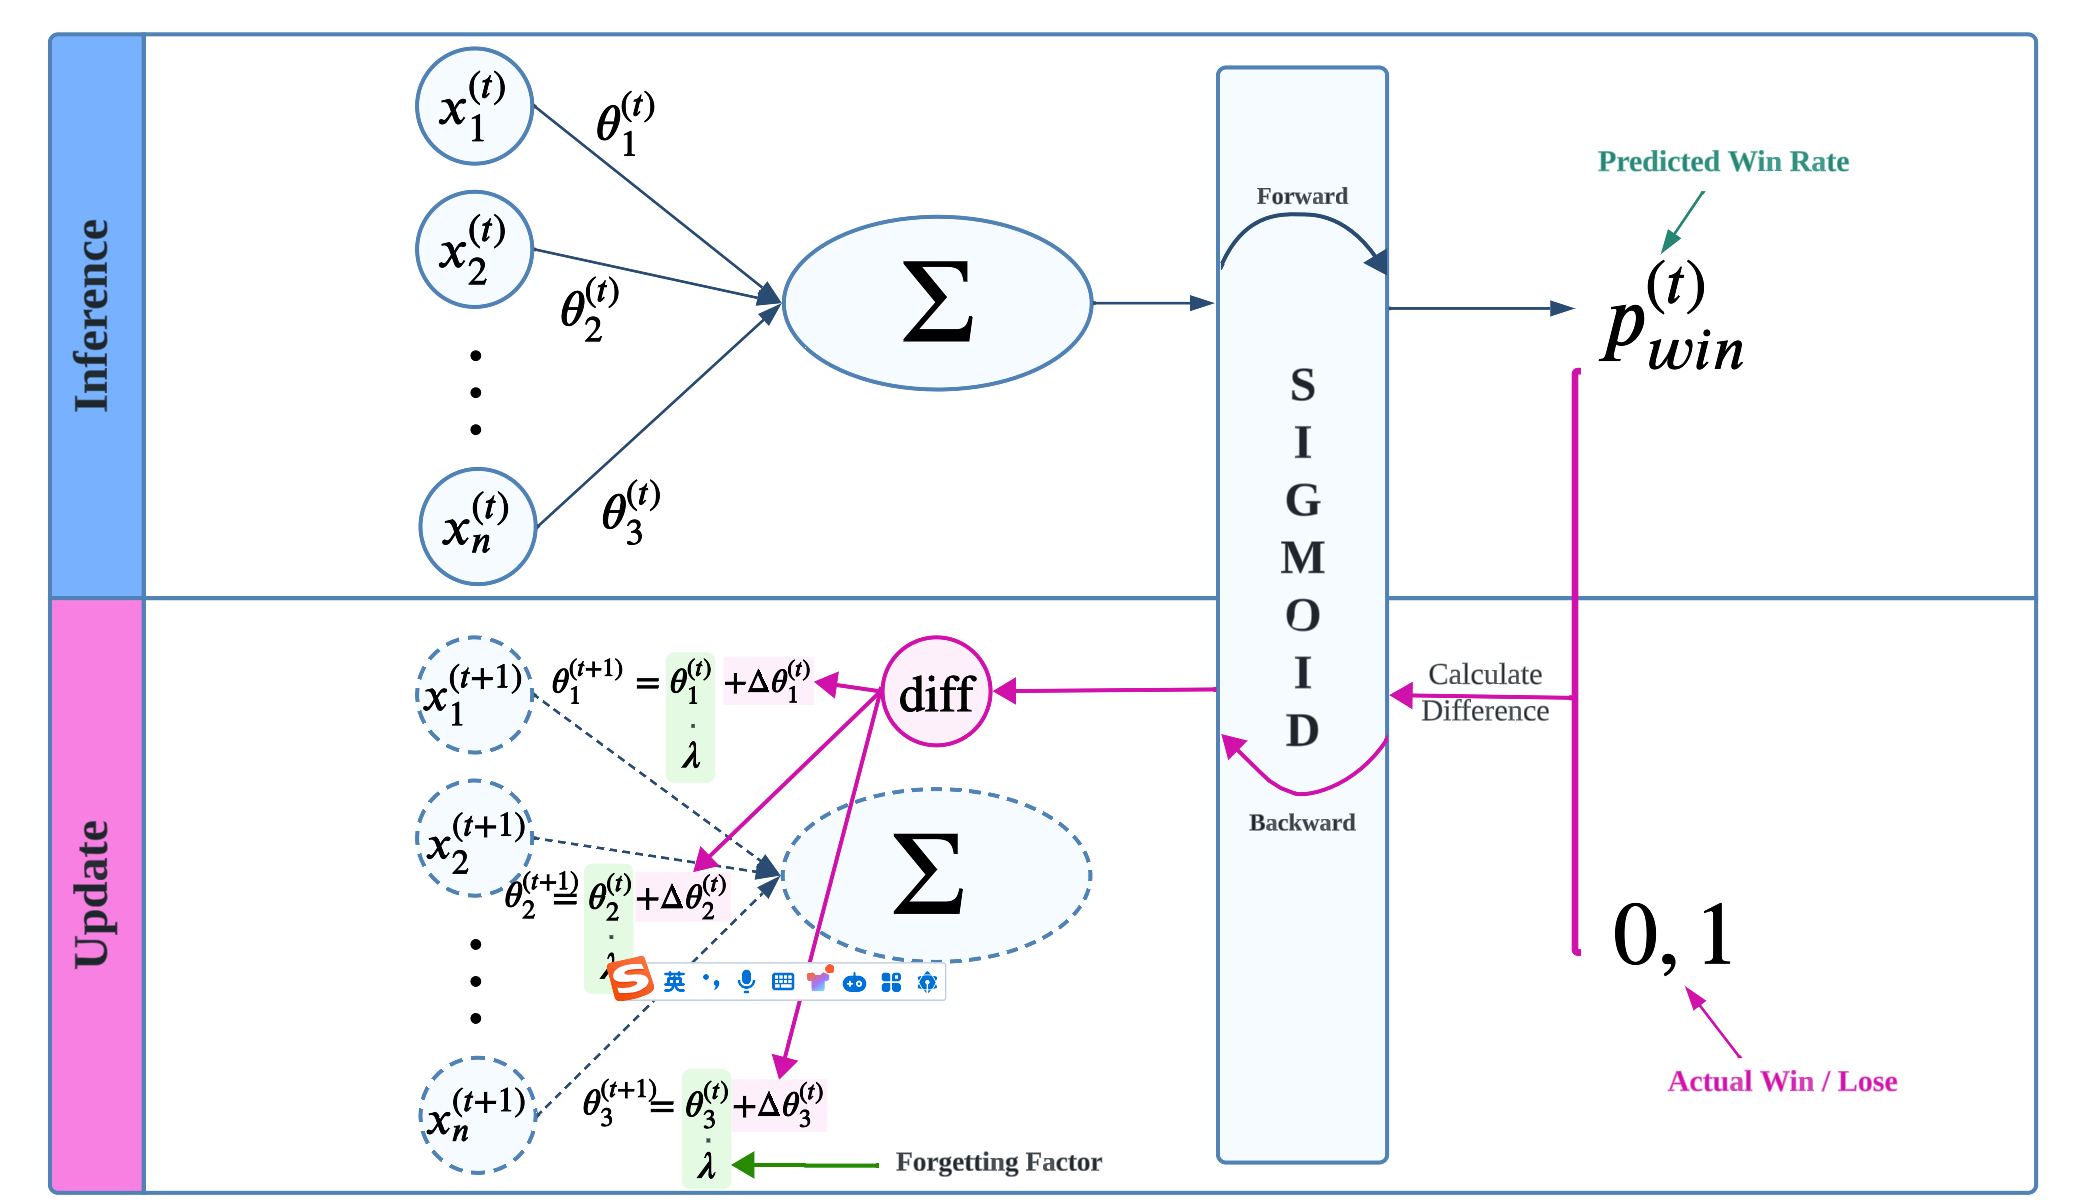
\includegraphics[width=.9\textwidth]{logistic.png} %图片的名称或者路径之中有空格会出问题 
	\caption{Process of the Progressive Logistic Regression Model} % 图片标题 
\end{figure}
\vspace{-0.8cm}

\subsubsection{Model Establishment}
Logistic regression is a statistical model used for binary classification problems, developed by David Cox in 1958. It is a type of generalized linear model (GLM) that uses a logistic function to model a binary dependent variable. The goal of logistic regression is to find the best fitting model to describe the relationship between the dichotomous characteristic of interest (dependent variable = 0 or 1) and a set of independent variables (predictors) \cite{5}. While the assumption of variable independence is ideal, logistic regression can still perform effectively in real-world scenarios where complete independence is rare, such as our feature set that describe match's information.

To feed the aggregated features into a logistic regression model, each feature set is represented as a vector $x^{(t)}$ at timestep t (which means the t-th point played in this match), and these vectors are used to calculate the probability of winning a point. $x^{(t)}$ is directly derived from the feature set \( F^{(t)} \), which contains both temporal features and non-temporal features.

The logistic regression model predicts the probability $ P(y^{(t)}=1|\mathbf{x}^{(t)}; \mathbf{\theta}) $
where $y^{(t)}=1$ indicates the event of interest (i.e., winning the point), $x^{(t)}$ is the feature vector at timestep t, and $\mathbf{\theta}$ represents the model parameter (weights). The model calculates the probability using the formula below:
\[
P(y^{(t)}=1|\mathbf{x}^{(t)}; \mathbf{\theta}) = \sigma(\mathbf{\theta}^\top \mathbf{x}^{(t)})
\]
where \( \sigma(z) \) is the sigmoid function defined as:
\[
\sigma(z) = \frac{1}{1 + e^{-z}}
\]
and \( z = \mathbf{\theta}^\top \mathbf{x}^{(t)} \) represents the linear combination of the features \( \mathbf{x}^{(t)} \) weighted by the model parameters \( \mathbf{\theta} \), expressed as:
\[
z = \theta_0 + \theta_1 x_1^{(t)} + \theta_2 x_2^{(t)} + \cdots + \theta_n x_n^{(t)}
\]
where \( \theta_0 \) is the intercept term, \( \theta_1, \theta_2, \ldots, \theta_n \) are the weights associated with each feature \( x_1^{(t)}, x_2^{(t)}, \ldots, x_n^{(t)} \) in the feature vector \( \mathbf{x}^{(t)} \).

Once we have the correct set of model parameters, we can determine the winning probability of a player based on the feature vector of the match for that player.


\subsubsection{Parameters Training \& Updating}
One of our Progressive Logistic Model's highlights is its ability to progressively adjust itself during the play of the match. But this does not mean it relies only on the real-time data; instead, we first train the model using the data given by the problem (pre-training phase), and when applied to a specific match, the progressive real-time data updates the parameters as the match unfolds (updating phase).

The training of the logistic regression model's parameters $\mathbf{\theta}$ is achieved by minimizing the logistic loss function, which quantifies the difference between the predicted outcomes and the actual results of matches:
\[
\mathcal{L}(\mathbf{\theta}) = -\frac{1}{m} \sum_{i=1}^{m} \left[ y^{(i)} \log(\sigma(\mathbf{\theta}^\top \mathbf{x}^{(i)})) + (1 - y^{(i)}) \log(1 - \sigma(\mathbf{\theta}^\top \mathbf{x}^{(i)})) \right]
\]
where \( m \) represents the number of observations in the training dataset, \( y^{(i)} \) denotes the outcome of the \( i \)-th point (win or loss), and \( \mathbf{x}^{(i)} \) is the feature vector associated with the \( i \)-th point in a match. Then, the parameter vector \( \mathbf{\theta} \) is optimized performed using Gradient Descent, described as:
\[
\mathbf{\theta} := \mathbf{\theta} - \alpha \nabla_{\mathbf{\theta}} \mathcal{L}(\mathbf{\theta})
\]
where \( \alpha \) is the learning rate that regulates the step size during each iteration, and \( \nabla_{\mathbf{\theta}} \mathcal{L}(\mathbf{\theta}) \) represents the gradient of the loss function with respect to the parameter vector \( \mathbf{\theta} \). Considering the constraints of the size of the dataset and the model's ability to update itself during a match, we meticulously choose different values for pre-training our model and updating our model during the match:
\[
\alpha = 
\begin{cases} 
	0.01 & \text{at pre-training phase } \\
	0.05 & \text{at updating phase } 
\end{cases}
\]
in this way, for each data point, both when pre-training and when updating, the parameter vector is iteratively updated in the direction that reduces the loss function.

At updating phase, the logistic regression model's parameters (\( \mathbf{\theta} \)) need to reflect the latest match data. This requires us to place more weight to the latest information of the points. Therefore, aside from using a higher learning rate value, a forgetting factor \( \lambda \) is incorporated into the parameter update rule:

\[
\mathbf{\theta}^{(t)} = \lambda \cdot \mathbf{\theta}^{(t-1)} +  \Delta\mathbf{\theta}^{(t-1)}
\]
\[ 
\Delta\mathbf{\theta}^{(t-1)} = - (1 - \lambda) \alpha \nabla_{\mathbf{\theta}^{(t-1)}} \mathcal{L}(\mathbf{\theta}^{(t-1)})
\]
this rule adjusts $\mathbf{\theta}^{(t)}$ by blending the previous parameters  \( \mathbf{\theta}^{(t-1)} \), scaled by \( \lambda \), with the changes dictated by new data (\( - \alpha \nabla_{\mathbf{\theta}^{(t-1)}} \mathcal{L}(\mathbf{\theta}^{(t-1)}) \)), scaled by $ (1 - \lambda) $. In such a way, the forgetting factor allows the model to prioritize recent information and adapt to changes in gameplay strategies or player performance over time.

To this point, we have thoroughly established our CourtSense model, which first uses feature selection combined with a sliding window mechanism, and leverages a Progressive Logistic Model to follow the flow of the match and predict the result of a specific point.

\subsubsection{Model Validation}
123

\subsubsection{Match Flow Visualization}



\subsubsection{Data Screening}
Judging from the map of Victoria in Figure 4 (right), the eastern region is mainly forest, while the western region is almost no forest. Furthermore, to demonstrate better the situa-tion of wildfires, we plot over a heat map in Figure 4 (left).
Considering the heat map we made, it shows the number of wildfires in various states of Victoria from 2012 to 2021, the darker the color, the greater number of fires. Although fires have also occurred in the western region, the number of eastern regions is much higher than that in the western region. 

\begin{figure}[htbp]
    \centering    
    \subfigure[Data Screening(left)]{				% 图片1([]内为子图标题)						
    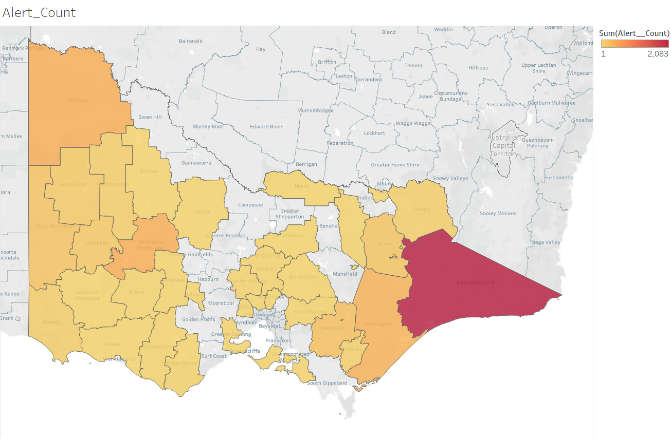
\includegraphics[width=0.45\textwidth]{Data_Screening(1).png}}			  % 子图1的图片宽度 不能空行
    \subfigure[Data Screening(right)]{				% 图片2
    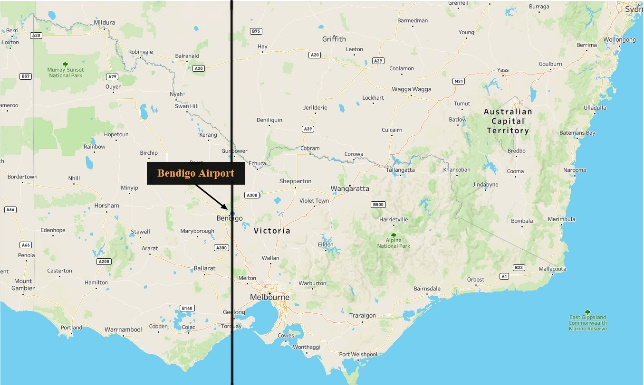
\includegraphics[width=0.45\textwidth]{Data_Screening(2).png}}
	\caption{Data Screening} % 图片标题 
\end{figure}

\begin{enumerate}[\bfseries 1.]
    \setlength{\parsep}{0ex} %段落间距
    \setlength{\topsep}{0ex} %列表到上下文的垂直距离
    \setlength{\itemsep}{0ex} %条目间距
    \item The analysis of locations of hovering VHF/UHF radio-repeater drones for fires can be more accurate if we have more complete data;
    \item The assumption that the "boots-on-the-ground" forward teams can be approximated as near the fire site is a bit idealized. If the trajectory of the team is taken into account, a more practical model and results can be obtained.
    \item Some approximate analysis methods are applied to model other places, which may lead to the situation that not to be the most optimal.
\end{enumerate}

\begin{algorithm}
	\caption{BLAH BLAH BLAH}
	\begin{algorithmic}[1] % The [1] option enables line numbering
		\REQUIRE wordlist, gameround, v, r, f
		\ENSURE bestguess
		\STATE $pguesses \gets []$
		\STATE $freq \gets modfreq(wordlist)$
		\FOR{$i \gets 1$ \TO $length(wordlist)$}
		\STATE $w \gets weightings(wordlist[i], freq, v, r, f)$
		\STATE $pguesses.append([w, wordlist[i]])$
		\ENDFOR
		\STATE $pguesses.sort(reverse = True)$
		\RETURN $pguesses[0][1]$
	\end{algorithmic}
\end{algorithm}

\[ \frac{{(x \cdot \gamma) \cdot \theta + 8}}{{6 \cdot \theta}} \tag{1}\]


\begin{table}[htbp]
	\begin{center}
		\caption{Data and Database Websites}
		\resizebox{\textwidth}{!}
		{\begin{tabular}{c c}
				\toprule[2pt]
				\multicolumn{1}{m{5cm}}{\centering \textbf{Database Names}}
				&\multicolumn{1}{m{10cm}}{\centering \textbf{Database Websites} }\\ %m后面是列宽
				\midrule
				Fire Alerts& https://www.globalforestwatch.org/map/ \\
				Altitude & https://search.earthdata.nasa.gov/search \\
				Latitude and Longitude & https://www.kaggle.com/carlosparadis/\\ 
				Google Scholar & https://scholar.google.com/ \\
				Maps& \copyright{} 2021 Mapbox \copyright{} OpenStreetMap\\
				\bottomrule[2pt]
		\end{tabular}}
	\end{center}
\end{table}



% F: References & Appendix

\clearpage   
\begin{thebibliography}{99}
    \bibitem{1} \href{https://www.skysports.com/tennis/news/32498/12920986/wimbledon-carlos-alcaraz-dismantles-daniil-medvedev-to-set-up-final-against-novak-djokovic}{Skysports | Wimbledon: Carlos Alcaraz dismantles Daniil Medvedev to set up final against Novak Djokovic.}
	\bibitem{2} \href{https://medium.com/swlh/cde03d99f410}{Medium | Predicting ATP Tennis Match Outcomes Using Serving Statistics.}
	\bibitem{3} \href{https://www.princeton.edu/~dixitak/home/Tennis.pdf}{Avinash Dixit, Susan Skeath. The Most Important Situations in Tennis – and in R\&D Competition.}
	\bibitem{4} \href{https://www.cis.upenn.edu/~bhusnur4/cit592\_fall2013/NeKe2005.pdf}{Pual K. Newton, Joseph B. Keller. Probability of Winning at Tennis I. Theory and Data.}
	\bibitem{5} \href{https://papers.tinbergen.nl/02119.pdf}{JS Cramer, University of Amsterdam, 2022. The Origins of Logistic Regression. }

\end{thebibliography}

\appendix
\section{Appendix I: The Genetic Algorithm}
blah,blah,blah

\section{Appendix II: Mail to the S.H.I.E.L.D}
blah,blah,blah





% Letter Page

\clearpage
\pagestyle{fancy}
\fancyhead{} % Clear all header fields
\begin{letter}{Letter to Central Intelligence Agency}
	\textbf{}\\
	\textbf{To:} Recipient Name \\
	\textbf{From:} Your Name \\
	\textbf{Subject:} The Subject of Your Letter \\
	\textbf{Date:} \today \\
	\textbf{}
	\begin{multicols}{2}
	We want to develop and summarize a model to classify solution words by difficulty.We constructed an AI
	simulating human thinking to solve problems based
	on iterative optimization parameter finding strategy.
	It could solve wordle about 3 times on average. We
	trained 450 such AI and took the average number of
	solving problems as the evaluation standard of difficulty. After that, we used k-means clustering algorithm
	to successfully classify normal problems and difficult
	problems, and found that normal problems generally
	have the characteristics of high word frequency, small
	number of non-repeating letters and so on.We also used
	correlation analysis to assess the relationship between
	the ai difficulty prediction and the average number
	of problems solved by humans, which showed a significant correlation. This verifies the accuracy of our
	model.
	Finally, we visualized the data and found an interesting conclusion: although daily reported results decreased, the proportion of difficult patterns increased.
	We attribute this to the presence of strong old players
	and a reluctance to post simple reports.We also found
	that the number of non-repeating letters also affected
	the percentage of hard mode.
	That’s all from our data analysis. I hope it’s helpful
	to your game. Thanks for watching.
	\end{multicols}
	
\end{letter}



% AI Report Page

\newcounter{savedpage}
\setcounter{savedpage}{\value{page}}

\includepdf[pages=-]{AIreport.pdf} 
\setcounter{page}{\value{savedpage}}

\end{document}  % 结束